\documentclass[
]{article}

\usepackage[utf8]{inputenc}

\author{
Ali Abuzaid\\Department of Mathematics, Al Azhar University -
Gaza \And Eyad Alkronz\\Department of Information Technology , Al azhar
University - Gaza
}
\title{}

\Plainauthor{Ali Abuzaid, Eyad Alkronz}


\Abstract{

}


%% publication information
%% \Volume{50}
%% \Issue{9}
%% \Month{June}
%% \Year{2012}
%% \Submitdate{}
%% \Acceptdate{2012-06-04}

\Address{
    }


% tightlist command for lists without linebreak
\providecommand{\tightlist}{%
  \setlength{\itemsep}{0pt}\setlength{\parskip}{0pt}}



\usepackage{booktabs}
\usepackage{longtable}
\usepackage{array}
\usepackage{multirow}
\usepackage{wrapfig}
\usepackage{float}
\usepackage{colortbl}
\usepackage{pdflscape}
\usepackage{tabu}
\usepackage{threeparttable}
\usepackage{threeparttablex}
\usepackage[normalem]{ulem}
\usepackage{makecell}
\usepackage{xcolor}

\usepackage{amsmath}

\begin{document}



\textbf{Abstract}

Outliers are values that differ significantly from the bulk of the data.
The existence of outliers can distort estimates and drastically impair
the performance and accuracy of a predictive model. Many statisticians
and data scientists have been drawn to the topic of outlier detection.
Outliers are dealt with one of three ways: accommodation, omission, or
winsorization.

Practitioners and data scientists employ several winsorization
statistics such as mean, median, mode and quantiles. This article
investigates the influence of these four winsorization statistics on the
estimations of parameters based on extensive simulation study.

Three probability distributions are considered namely: normal, negative
binomial, and exponential with different levels of contamination.
Furthermore, bias, mean square error, and proportion of fitted
winsorizated samples are obtained as indicators of performance.

The simulation findings demonstrate that winsorizing outliers in
symmetric distributions by any of the location parameters leads to a
better estimate, however using the median outperforms other statistics
in asymmetric distributions. Furthermore, as the contamination level is
decreased or the sample size is increased, the estimations improve.

For illustration purposes, a real data of internet usage session
duration for 4500 users with more than 2 million records are fitted for
the exponential distribution and the detected outliers were winsorizated
by the considered statistics.

\textbf{Keywords} Capping; flooring; outlier; quantile-based.

\hypertarget{introduction}{%
\section{Introduction}\label{introduction}}

Outliers are values in data that differ extremely from a major sample of
the data, the presence of outliers can bias the estimates and, as a
consequence, significantly reduce the performance and accuracy of a
predictable model. The problem of outlier-detection has attracted the
attention of many statisticians and data scientists.

The methods of outlier-detection are broadly classified into different
classes, namely distribution-based methods, depth-based methods, and
density-based methods (Preparata and Shamos, 1988, Dominguesa, et al
2018).

The argument on the handling of outliers is continued between the belief
of Tukey (1959) that rejecting outliers indiscriminately is
inappropriate, and other various trimming and winsorization techniques.
Thus, after detection, outliers are handled in one of three ways:
accommodation, omission, or winsorization.

The accommodation is utilized by robust statistical methods in order to
resist the effect of outliers on the parameter estimates (Ekezie \& Ogu,
2013), which indirectly destroy the conclusions of the study (Hubert et
al., 2008, Farcomeni \& Ventura, 2010). Trimming of outliers has been
well studied, where (Lix and Keselman, 1998; Yusof et al.~2013) have
proved its beneficial in terms of robustness, while the type (symmetric
or asymmetric) and percentage of trimming have been discussed by (Babu
et al.~1999; Wilcox, 2003).

In winsorization, the extreme values are replaced by other appropriate
values to reduce the effect of the outliers on the estimation and
modeling power (Frey, 2018). The choose of winsorization percentage
cut-off point as well as the winsorization statistic are challenging. A
poor choice of winsorization percentage will inflated the mean squared
errors (MSE) of desired estimators. Thus, it is recommended to the
choose cut-off point that minimizes the MSE compared to the classical
estimator.

In the context of data science, practitioners used different statistics
for winsorization, such as mean, median and quantiles. To the best of
our knowledge, no study has been published dealing with the impact of
different winsorization statistics on the estimators. This article
investigates the impact of four winsorization statistics viz mean,
median, mode and Quantile-based Flooring and Capping technique on the
estimates of parameters of three distributions, namely normal, negative
binomial and exponential distributions.

The rest of this article is organized as follows: Section 2 reviews the
source, impact, detection and winsorization of outlies. Section 3
investigates the impact of winsorization methods on the parameters
estimates, and Section 4 illustrates the considered methods on real
data.

\hypertarget{outliers-and-winsorization}{%
\section{Outliers and Winsorization}\label{outliers-and-winsorization}}

\hypertarget{sources-and-impact-of-outliers}{%
\subsection{Sources and Impact of
Outliers}\label{sources-and-impact-of-outliers}}

Observed variables often contain outliers that differ extremely from a
major sample of the data. Some data sets may come from homogeneous
groups; others from heterogeneous groups that have different
characteristics regarding a specific variable, Outliers can be caused by
incorrect measurements, including data entry errors, or by sampling from
a different population than the rest of the data (Frost, 2020).

Outliers may cause a negative effect on data analyses such as biasing
the estimation, reduce the predictability of constructed model, or it
may provide useful information about data when we look into an unusual
response to a given study. The data must be evaluated for the presence
of outliers before beginning the procedure with the main bulk of data.
Thus, outlier detection is an important part of data analysis in the
above two cases.

\hypertarget{outliers-detection}{%
\subsection{Outliers Detection}\label{outliers-detection}}

There are different methods for identifying outliers, including square
root transformation, median absolute deviation, Grubb's test, Ueda's
method as explained recently by (Shimizu, 2022). In this article we are
going to use Tukey's method boxplot (Tukey, 1977); due to its popularity
and less sensitivity of outliers' existence compare to other tests.

Boxplot is a well-known simple graphical tool to display information
about continuous univariate data based on five summaries, namely,
median, lower quartile \(Q_1\), upper quartile \(Q_3\), lower extreme,
and upper extreme of a data set. It is less sensitive to extreme values
of the data than the previous methods using the sample mean and standard
variance because it uses quartiles which are resistant to extreme
values. The rule of the method is that any value smaller than the lower
fence \(L_F=Q_1 - \nu*IQR\) or larger than the upper fence
\(U_F=Q_3+ \nu*IQR\) is a possible outlier, where \(\nu\) is the
resistance factor and \(IQR=Q_3 -Q_1\) is the interquartile range..

Different values of \(\nu\) can be considered, but the nominal value is
\(\nu=1.5\) (Hoaglin, et al, 1986). Various versions of the boxplot were
also proposed (See Abuzaid et al; 2012, Saeger et al; 2016).

The following subsection discusses the treatment of outliers via
winsorization.

\hypertarget{winsorization-of-outliers}{%
\subsection{Winsorization of outliers}\label{winsorization-of-outliers}}

There are two common methods for treating outliers in a data set. The
first is to remove outliers as a means of trimming the data set. The
second method involves replacing the values of outliers with suitable
statistic such as mean, median, mode or quantile-based technique as
follows:

\(1.\ Replace\ outliers\ by\ mean:\) In this technique outliers are
replaced with the arithmetic mean \(\bar{x}=\sum_{i=1}^n \frac{x_i}{n}\)
of the remaining observations after removing outliers.

\(2.\ Replace\ outliers\ by\ median:\) The median value that is the
middle value in an ordered remaining observations
\[Q_2 =\bigg\{ \begin{aligned} 
 &x_{\frac {n+1}{2}}  \,\,\,\,\,\,\,\,\,\,\,\,\,\,\,\,\,\,\,\,\,\,\,\,\,\,\,\,\,\,\,\,\,\,\,\,\,\, \text{if $n$ is odd}  \nonumber\\   
 &\big(x_{\frac {n}{2}} + x_{\frac {n}{2}+1} \big)/2 \,\,\,\,\,\,\,\,\,\,\, \text{if $n$ is even} \nonumber
\end{aligned}\]

is used to replace the detected outliers.

\(3.\ Replace \ outliers \ by \ mode:\) The outliers are replaced with
the mode value of the remaining observations, which is appears most
often in a set of data values.

\(4.\ Quantile-based \ Flooring \ and \ Capping:\) in this
quantile-based technique, the maximum outliers are replaced with upper
fence \(U_F\) (capped), and the minimum outliers are replaced with lower
fence \(L_F\) (floored).

The following section investigates the effect of the four considered
winsorization statistics on the performance of parameter estimates for
different probability distributions via Monte carlo simulation.

\hypertarget{simulation-numerical-study}{%
\section{Simulation (Numerical
Study)}\label{simulation-numerical-study}}

An R code has been developed and implemented in \(R\) Studio environment
to generate random data sets from three different probability
distributions namely, normal, negative binomial and exponential
distribution.

\hypertarget{settings-of-data-generation}{%
\subsection{Settings of Data
Generation}\label{settings-of-data-generation}}

Data were generated with four different sample sizes, \(n\) = 20,50,100
and 200, in such a way that (\(1-\epsilon\)) of data are generated from
the original distribution (\(P\)) and the rest \(\epsilon\) of data are
generated from the contamination distribution (\(Q\)). Thus, the
contaminated data structure can be formulated as
\(P_{\epsilon}=(1-\epsilon)P+\epsilon Q\), where \(\epsilon\) is the
contamination level and \(\epsilon\) =0.05, 0.10 or 0.15.The following
three probability distributions are considered:

\hypertarget{normal-distribution}{%
\subsubsection{Normal distribution}\label{normal-distribution}}

For normal random variable, \(X\sim N(\mu,\sigma^2)\); data were
generated from the standard normal distribution with \(\mu = 0\) and
\(\sigma = 1\). For contamination procedure; the contaminated data were
generated from another normal distribution with \(\mu = 4\) and
\(\sigma = 2\).

The maximum likelihood estimator (\(MLE\)) of the mean and standard
deviation are obtained as the sample mean
\(\hat{\mu}_{mle} = \bar{x} = \frac{1}{n} \sum_{i=1}^n x_i\),and
\(\hat{\sigma} = \sqrt{\frac{\sum (x_{i} - \bar{x})^{2}}{n - 1}}\),
respectively.

\hypertarget{negative-binomial-distribution}{%
\subsubsection{Negative binomial
distribution}\label{negative-binomial-distribution}}

Random variable \(X\) follows the negative binomial distribution
\(X \sim NB(k,p)\) with mean \(\mu =\frac{k}{p}\) and variance
\(\sigma^2= \frac{k(1-p)}{p^2}\) if \(X\) is the count of independent
Bernoulli trials required to achieve the \(k^{th}\) successful trials
when the probability of success is a constant \(p\). The probability of
\(x=n\) trials is \(f(X=n)= {n-1 \choose k-1} p^k (1-p)^{n-k}\). The
\(MLE\) of \(p\) is given by: \(\hat{p} = \frac{k}{x + k}\).

For negative binomial random variable; data are generated with
parameters \(k=2\) and \(p=0.2\), while the contaminated data are
generated from Poisson distribution with \(\lambda = 32\), where the
probability of \(k\) successes is
\(P(X=k) = \frac {(e^{-\lambda} \lambda^k)} {k!}\).

\hypertarget{exponential-distribution}{%
\subsubsection{Exponential
distribution}\label{exponential-distribution}}

The Exponential distribution is the most commonly used model in
reliability and life-testing analysis, (i.e
\(f(x)=\theta e^{-\theta x}\) for \(x \geq 0\)). The \(MLE\) of
\(\theta\) is given by \(\hat{\theta}= \frac{1}{\bar{x}}\).\\
Data were generated with parameter \(\theta = 0.5\), and the
contaminated data were generated from exponential distribution with
\(\theta = 0.05\).

For each combination of the considered probability distributions,sample
sizes, contamination levels and winsorization statistics; the generation
procedures are repeated 1000 iterations to ensure the convergence.

\hypertarget{performance-indicators}{%
\subsection{Performance indicators}\label{performance-indicators}}

The impact of the considered four outliers winsorization statistics on
the parameter estimates are assessed by three common indicators as
follows:

\begin{enumerate}
\def\labelenumi{\arabic{enumi}.}
\item
  \(Bias\), is the difference between the estimator's expected value and
  the true value of the parameter being estimated.
\item
  \(Mean \ Square\ Error (MSE)\), is a measure of the quality of an
  estimator. As it is derived from the square of Euclidean distance, it
  is always a positive value that decreases as the error approaches
  zero. \(MSE = \frac{1}{n} \sum_{i=1}^n (\beta - \hat{\beta})^2\) where
  \(\beta\) and \(\hat{\beta}\) are the true and estimated values of the
  considered parameters .
\item
  \(Goodness\ of\ fit\ tests\), are statistical tests aiming to
  determine whether a set of observed values match those expected under
  the applicable distribution. There are different goodness-of-fit
  tests, in this article the Shipiro-Wilk test is used in the case of
  normal and exponential distributions, while Kolmogorov-Smirnov test is
  used in the case of negative binomial distribution.
\end{enumerate}

\hypertarget{results}{%
\subsection{Results}\label{results}}

Simulation results are summarized in Tables (1-5) and show that,
regardless the distribution, contamination level or winsorization
statistics, the results of simulation studies reveal that, the
performance of parameter estimates are improved as the sample size
increased, where the MSE has a decreasing function with the sample size,
and the bias has a decreasing function of the sample size for
\(n\)\textless100 and constant function for \(n\)\textgreater100, as
partially presented in Figure 1.

The performance has relatively an inverse relationship with the
contamination level \(\epsilon\).

For normal distribution, due to its symmetric nature the mean, median
and mode winsorization statistics have almost similar effect on the
parameters estimates (i.e.~\(\mu\) and \(\sigma^2\)), while they
outperform the quantile-based winsorization statistic as given in Tables
(1-2).

For negative binomial case, the mode winsorization statistic outperforms
the other winsorization statistics for higher levels of contamination
\(\epsilon=0.15\), while the mean winsorization statistic performs
better than other winsorization statistics for smaller levels of
contamination \((\epsilon<0.15)\) as presented in Table 3.

For the exponential distribution (Table 4), the mean winsorization
statistic has the best performance followed by median, mode and then the
quantile-based method. This behavior may be referred to the MLE
estimator of the \(\theta\), which is mainly the sample mean.

\begin{CodeChunk}


\begin{center}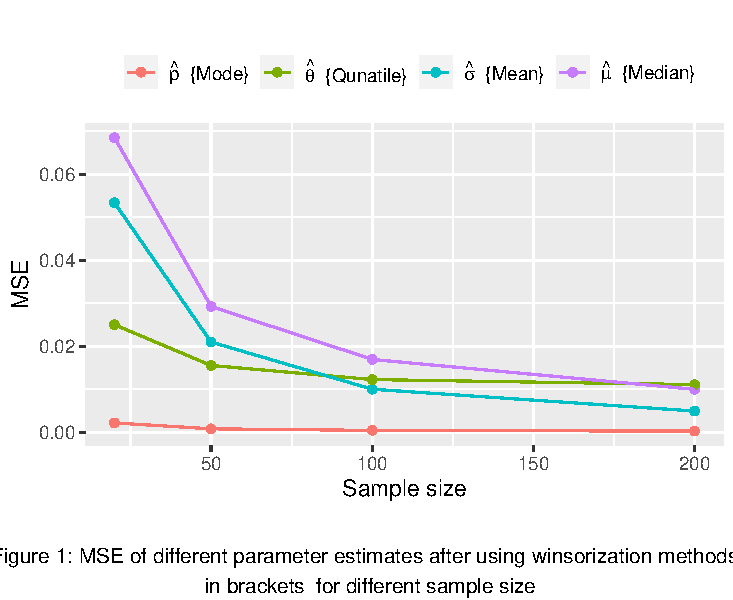
\includegraphics{new_header_format_files/figure-latex/unnamed-chunk-3-1} \end{center}

\end{CodeChunk}

From the prospective of goodness of fits test, as shown in Table 5, in
the case of normal distribution, mean, median and mode winsorization
statistics have consistent performance with respect to the contamination
level and sample size, where the proportion of samples fitted by normal
distribution close to 1 when the contamination level is
\(\epsilon=0.05\). In the case of an exponential distribution, all
considered winsorization statistics perform approximately equally and
perfectly, where the proportion of samples fitted by exponential
distribution close to 1 regardless the sample size or contamination
level.\\
The proportions of fitted samples by negative binomial are less than the
other two distributions. The quantile-based winsorization statistic the
worst performance compare to other three considered statistics because
it accumulates the winsorizated values at the edges of distribution and
malforms the nature of distribution. Thus, the mean winsorization
statistic is recommended for most of the cases especially for smaller
levels of contamination.

\begin{CodeChunk}
\begin{table}[H]

\caption{\label{tab:unnamed-chunk-4}Bias (MSE) of the normal distribution's mean estimator for different winsorization methods}
\centering
\begin{tabular}[t]{l|l|l|l|l|l}
\hline
\multicolumn{2}{c|}{ } & \multicolumn{4}{c}{Winsorization Methods} \\
\cline{3-6}
n & $\epsilon$ & Quantile-based & Mean & Median & Mode\\
\hline
\cellcolor{gray!6}{20} & \cellcolor{gray!6}{5} & \cellcolor{gray!6}{0.111 (0.06)} & \cellcolor{gray!6}{0.021 (0.058)} & \cellcolor{gray!6}{0.02 (0.058)} & \cellcolor{gray!6}{0.02 (0.058)}\\
\hline
50 & 5 & 0.092 (0.027) & 0.019 (0.021) & 0.019 (0.021) & 0.019 (0.021)\\
\hline
\cellcolor{gray!6}{100} & \cellcolor{gray!6}{5} & \cellcolor{gray!6}{0.122 (0.025)} & \cellcolor{gray!6}{0.029 (0.012)} & \cellcolor{gray!6}{0.029 (0.012)} & \cellcolor{gray!6}{0.028 (0.012)}\\
\hline
200 & 5 & 0.12 (0.02) & 0.027 (0.007) & 0.027 (0.007) & 0.026 (0.007)\\
\hline
\cellcolor{gray!6}{20} & \cellcolor{gray!6}{10} & \cellcolor{gray!6}{0.24 (0.111)} & \cellcolor{gray!6}{0.074 (0.068)} & \cellcolor{gray!6}{0.074 (0.068)} & \cellcolor{gray!6}{0.074 (0.069)}\\
\hline
50 & 10 & 0.245 (0.081) & 0.068 (0.029) & 0.067 (0.029) & 0.066 (0.029)\\
\hline
\cellcolor{gray!6}{100} & \cellcolor{gray!6}{10} & \cellcolor{gray!6}{0.244 (0.07)} & \cellcolor{gray!6}{0.068 (0.017)} & \cellcolor{gray!6}{0.066 (0.017)} & \cellcolor{gray!6}{0.065 (0.017)}\\
\hline
200 & 10 & 0.245 (0.065) & 0.064 (0.01) & 0.062 (0.01) & 0.061 (0.01)\\
\hline
\cellcolor{gray!6}{20} & \cellcolor{gray!6}{15} & \cellcolor{gray!6}{0.353 (0.18)} & \cellcolor{gray!6}{0.113 (0.08)} & \cellcolor{gray!6}{0.111 (0.08)} & \cellcolor{gray!6}{0.108 (0.082)}\\
\hline
50 & 15 & 0.399 (0.182) & 0.14 (0.049) & 0.136 (0.048) & 0.132 (0.048)\\
\hline
\cellcolor{gray!6}{100} & \cellcolor{gray!6}{15} & \cellcolor{gray!6}{0.378 (0.154)} & \cellcolor{gray!6}{0.121 (0.028)} & \cellcolor{gray!6}{0.117 (0.027)} & \cellcolor{gray!6}{0.113 (0.026)}\\
\hline
200 & 15 & 0.378 (0.149) & 0.119 (0.022) & 0.115 (0.021) & 0.111 (0.02)\\
\hline
\end{tabular}
\end{table}

\end{CodeChunk}

\begin{CodeChunk}
\begin{table}[H]

\caption{\label{tab:unnamed-chunk-5}Bias (MSE) of the normal distribution's standared deviation estimator for different winsorization methods}
\centering
\begin{tabular}[t]{l|l|l|l|l|l}
\hline
\multicolumn{2}{c|}{ } & \multicolumn{4}{c}{Winsorization  Methods} \\
\cline{3-6}
n & $\epsilon$ & Quantile-based & Mean & Median & Mode\\
\hline
\cellcolor{gray!6}{20} & \cellcolor{gray!6}{5} & \cellcolor{gray!6}{0.095 (0.047)} & \cellcolor{gray!6}{0.078 (0.05)} & \cellcolor{gray!6}{0.077 (0.05)} & \cellcolor{gray!6}{0.072 (0.049)}\\
\hline
50 & 5 & 0.094 (0.022) & 0.032 (0.017) & 0.032 (0.017) & 0.029 (0.016)\\
\hline
\cellcolor{gray!6}{100} & \cellcolor{gray!6}{5} & \cellcolor{gray!6}{0.125 (0.023)} & \cellcolor{gray!6}{0.026 (0.01)} & \cellcolor{gray!6}{0.026 (0.01)} & \cellcolor{gray!6}{0.024 (0.01)}\\
\hline
200 & 5 & 0.123 (0.019) & 0.023 (0.005) & 0.023 (0.005) & 0.022 (0.005)\\
\hline
\cellcolor{gray!6}{20} & \cellcolor{gray!6}{10} & \cellcolor{gray!6}{0.226 (0.101)} & \cellcolor{gray!6}{0.014 (0.053)} & \cellcolor{gray!6}{0.013 (0.053)} & \cellcolor{gray!6}{0.007 (0.053)}\\
\hline
50 & 10 & 0.25 (0.081) & 0.005 (0.021) & 0.005 (0.021) & 0.001 (0.021)\\
\hline
\cellcolor{gray!6}{100} & \cellcolor{gray!6}{10} & \cellcolor{gray!6}{0.252 (0.073)} & \cellcolor{gray!6}{0.006 (0.01)} & \cellcolor{gray!6}{0.006 (0.01)} & \cellcolor{gray!6}{0.009 (0.01)}\\
\hline
200 & 10 & 0.255 (0.07) & 0.005 (0.005) & 0.005 (0.005) & 0.007 (0.005)\\
\hline
\cellcolor{gray!6}{20} & \cellcolor{gray!6}{15} & \cellcolor{gray!6}{0.35 (0.183)} & \cellcolor{gray!6}{0.004 (0.064)} & \cellcolor{gray!6}{0.005 (0.064)} & \cellcolor{gray!6}{0.015 (0.065)}\\
\hline
50 & 15 & 0.401 (0.188) & 0.062 (0.036) & 0.063 (0.036) & 0.069 (0.036)\\
\hline
\cellcolor{gray!6}{100} & \cellcolor{gray!6}{15} & \cellcolor{gray!6}{0.387 (0.162)} & \cellcolor{gray!6}{0.048 (0.016)} & \cellcolor{gray!6}{0.049 (0.016)} & \cellcolor{gray!6}{0.053 (0.016)}\\
\hline
200 & 15 & 0.392 (0.159) & 0.055 (0.01) & 0.055 (0.01) & 0.059 (0.01)\\
\hline
\end{tabular}
\end{table}

\end{CodeChunk}

\begin{CodeChunk}
\begin{table}[H]

\caption{\label{tab:unnamed-chunk-6}Bias (MSE) of the negative binomial distribution probability of success estimator for different winsorization methods}
\centering
\begin{tabular}[t]{l|l|l|l|l|l}
\hline
\multicolumn{2}{c|}{ } & \multicolumn{4}{c}{Winsorization methods} \\
\cline{3-6}
n & $\epsilon$ & Quantile-based & Mean & Median & Mode\\
\hline
\cellcolor{gray!6}{20} & \cellcolor{gray!6}{5} & \cellcolor{gray!6}{0.013 (0.001)} & \cellcolor{gray!6}{0.017 (0.002)} & \cellcolor{gray!6}{0.018 (0.002)} & \cellcolor{gray!6}{0.019 (0.002)}\\
\hline
50 & 5 & 0.014 (0) & 0.011 (0.001) & 0.012 (0.001) & 0.014 (0.001)\\
\hline
\cellcolor{gray!6}{100} & \cellcolor{gray!6}{5} & \cellcolor{gray!6}{0.017 (0)} & \cellcolor{gray!6}{0.01 (0)} & \cellcolor{gray!6}{0.011 (0)} & \cellcolor{gray!6}{0.014 (0.001)}\\
\hline
200 & 5 & 0.018 (0) & 0.008 (0) & 0.01 (0) & 0.013 (0)\\
\hline
\cellcolor{gray!6}{20} & \cellcolor{gray!6}{10} & \cellcolor{gray!6}{0.031 (0.001)} & \cellcolor{gray!6}{0.005 (0.002)} & \cellcolor{gray!6}{0.007 (0.002)} & \cellcolor{gray!6}{0.009 (0.002)}\\
\hline
50 & 10 & 0.034 (0.001) & 0.001 (0.001) & 0.003 (0.001) & 0.006 (0.001)\\
\hline
\cellcolor{gray!6}{100} & \cellcolor{gray!6}{10} & \cellcolor{gray!6}{0.034 (0.001)} & \cellcolor{gray!6}{0.002 (0)} & \cellcolor{gray!6}{0 (0)} & \cellcolor{gray!6}{0.004 (0)}\\
\hline
200 & 10 & 0.034 (0.001) & 0.001 (0) & 0.001 (0) & 0.006 (0)\\
\hline
\cellcolor{gray!6}{20} & \cellcolor{gray!6}{15} & \cellcolor{gray!6}{0.045 (0.002)} & \cellcolor{gray!6}{0.006 (0.002)} & \cellcolor{gray!6}{0.004 (0.002)} & \cellcolor{gray!6}{0.001 (0.002)}\\
\hline
50 & 15 & 0.049 (0.002) & 0.019 (0.001) & 0.017 (0.001) & 0.015 (0.001)\\
\hline
\cellcolor{gray!6}{100} & \cellcolor{gray!6}{15} & \cellcolor{gray!6}{0.047 (0.002)} & \cellcolor{gray!6}{0.015 (0.001)} & \cellcolor{gray!6}{0.013 (0.001)} & \cellcolor{gray!6}{0.009 (0.001)}\\
\hline
200 & 15 & 0.046 (0.002) & 0.016 (0) & 0.014 (0) & 0.01 (0)\\
\hline
\end{tabular}
\end{table}

\end{CodeChunk}

\begin{CodeChunk}
\begin{table}[H]

\caption{\label{tab:unnamed-chunk-7}Bias (MSE) of the exponential distribution's rate estimator for different winsorization methods}
\centering
\begin{tabular}[t]{l|l|l|l|l|l|l}
\hline
\multicolumn{3}{c|}{ } & \multicolumn{4}{c}{Winsorization Methods} \\
\cline{4-7}
n & $\epsilon$ & Before & Quantile-based & Mean & Median & Mode\\
\hline
\cellcolor{gray!6}{20} & \cellcolor{gray!6}{5} & \cellcolor{gray!6}{0.359 (0.13)} & \cellcolor{gray!6}{0.069 (0.017)} & \cellcolor{gray!6}{0.077 (0.033)} & \cellcolor{gray!6}{0.092 (0.037)} & \cellcolor{gray!6}{0.115 (0.045)}\\
\hline
50 & 5 & 0.309 (0.096) & 0.039 (0.007) & 0.08 (0.018) & 0.093 (0.021) & 0.116 (0.028)\\
\hline
\cellcolor{gray!6}{100} & \cellcolor{gray!6}{5} & \cellcolor{gray!6}{0.335 (0.113)} & \cellcolor{gray!6}{0.045 (0.004)} & \cellcolor{gray!6}{0.07 (0.01)} & \cellcolor{gray!6}{0.082 (0.012)} & \cellcolor{gray!6}{0.107 (0.018)}\\
\hline
200 & 5 & 0.329 (0.109) & 0.043 (0.003) & 0.066 (0.007) & 0.078 (0.009) & 0.104 (0.014)\\
\hline
\cellcolor{gray!6}{20} & \cellcolor{gray!6}{10} & \cellcolor{gray!6}{0.382 (0.147)} & \cellcolor{gray!6}{0.13 (0.025)} & \cellcolor{gray!6}{0.055 (0.024)} & \cellcolor{gray!6}{0.076 (0.029)} & \cellcolor{gray!6}{0.106 (0.038)}\\
\hline
50 & 10 & 0.376 (0.142) & 0.108 (0.016) & 0.052 (0.012) & 0.07 (0.015) & 0.103 (0.022)\\
\hline
\cellcolor{gray!6}{100} & \cellcolor{gray!6}{10} & \cellcolor{gray!6}{0.375 (0.141)} & \cellcolor{gray!6}{0.102 (0.012)} & \cellcolor{gray!6}{0.051 (0.007)} & \cellcolor{gray!6}{0.069 (0.009)} & \cellcolor{gray!6}{0.103 (0.016)}\\
\hline
200 & 10 & 0.374 (0.14) & 0.101 (0.011) & 0.047 (0.004) & 0.063 (0.006) & 0.098 (0.012)\\
\hline
\cellcolor{gray!6}{20} & \cellcolor{gray!6}{15} & \cellcolor{gray!6}{0.395 (0.157)} & \cellcolor{gray!6}{0.179 (0.038)} & \cellcolor{gray!6}{0.038 (0.018)} & \cellcolor{gray!6}{0.064 (0.022)} & \cellcolor{gray!6}{0.1 (0.032)}\\
\hline
50 & 15 & 0.38 (0.145) & 0.151 (0.026) & 0.042 (0.01) & 0.065 (0.013) & 0.103 (0.022)\\
\hline
\cellcolor{gray!6}{100} & \cellcolor{gray!6}{15} & \cellcolor{gray!6}{0.393 (0.155)} & \cellcolor{gray!6}{0.159 (0.026)} & \cellcolor{gray!6}{0.03 (0.004)} & \cellcolor{gray!6}{0.053 (0.007)} & \cellcolor{gray!6}{0.096 (0.014)}\\
\hline
200 & 15 & 0.393 (0.154) & 0.156 (0.025) & 0.029 (0.003) & 0.051 (0.005) & 0.095 (0.012)\\
\hline
\end{tabular}
\end{table}

\end{CodeChunk}

\begin{CodeChunk}
\begin{table}[H]

\caption{\label{tab:unnamed-chunk-8}The proportion of fitted samples by associated distributions at 0.05 level of significance after winsorizing outliers.}
\centering
\begin{tabular}[t]{l|l|c|c|c|c|l|l|c|c|c|c|l|l}
\hline
\multicolumn{2}{c|}{Distribution} & \multicolumn{4}{c|}{Normal distribution} & \multicolumn{4}{c|}{Exponential distribution} & \multicolumn{4}{c}{Negative binomial distribution} \\
\cline{1-2} \cline{3-6} \cline{7-10} \cline{11-14}
n & $\epsilon$ & Qun & Mean & Med & Mode & Qun & Mean & Med & Mode & Qun & Mean & Med & Mode\\
\hline
\cellcolor{gray!6}{20} & \cellcolor{gray!6}{5} & \cellcolor{gray!6}{0.961} & \cellcolor{gray!6}{0.970} & \cellcolor{gray!6}{0.949} & \cellcolor{gray!6}{0.924} & \cellcolor{gray!6}{0.999} & \cellcolor{gray!6}{1.000} & \cellcolor{gray!6}{0.996} & \cellcolor{gray!6}{0.984} & \cellcolor{gray!6}{0.748} & \cellcolor{gray!6}{0.912} & \cellcolor{gray!6}{0.878} & \cellcolor{gray!6}{0.848}\\
\hline
50 & 5 & 0.926 & 0.970 & 0.965 & 0.958 & 1.000 & 1.000 & 1.000 & 0.997 & 0.442 & 0.682 & 0.606 & 0.538\\
\hline
\cellcolor{gray!6}{100} & \cellcolor{gray!6}{5} & \cellcolor{gray!6}{0.614} & \cellcolor{gray!6}{0.968} & \cellcolor{gray!6}{0.960} & \cellcolor{gray!6}{0.934} & \cellcolor{gray!6}{1.000} & \cellcolor{gray!6}{1.000} & \cellcolor{gray!6}{1.000} & \cellcolor{gray!6}{1.000} & \cellcolor{gray!6}{0.294} & \cellcolor{gray!6}{0.450} & \cellcolor{gray!6}{0.418} & \cellcolor{gray!6}{0.356}\\
\hline
200 & 5 & 0.137 & 0.962 & 0.953 & 0.916 & 1.000 & 1.000 & 1.000 & 1.000 & 0.152 & 0.254 & 0.200 & 0.198\\
\hline
\cellcolor{gray!6}{20} & \cellcolor{gray!6}{10} & \cellcolor{gray!6}{0.873} & \cellcolor{gray!6}{0.951} & \cellcolor{gray!6}{0.939} & \cellcolor{gray!6}{0.910} & \cellcolor{gray!6}{0.997} & \cellcolor{gray!6}{0.998} & \cellcolor{gray!6}{0.986} & \cellcolor{gray!6}{0.964} & \cellcolor{gray!6}{0.582} & \cellcolor{gray!6}{0.846} & \cellcolor{gray!6}{0.792} & \cellcolor{gray!6}{0.782}\\
\hline
50 & 10 & 0.474 & 0.938 & 0.918 & 0.879 & 0.998 & 0.999 & 0.996 & 0.984 & 0.256 & 0.542 & 0.488 & 0.380\\
\hline
\cellcolor{gray!6}{100} & \cellcolor{gray!6}{10} & \cellcolor{gray!6}{0.060} & \cellcolor{gray!6}{0.890} & \cellcolor{gray!6}{0.873} & \cellcolor{gray!6}{0.805} & \cellcolor{gray!6}{0.998} & \cellcolor{gray!6}{1.000} & \cellcolor{gray!6}{1.000} & \cellcolor{gray!6}{0.998} & \cellcolor{gray!6}{0.090} & \cellcolor{gray!6}{0.352} & \cellcolor{gray!6}{0.314} & \cellcolor{gray!6}{0.234}\\
\hline
200 & 10 & 0.000 & 0.777 & 0.752 & 0.664 & 1.000 & 1.000 & 1.000 & 0.997 & 0.008 & 0.258 & 0.192 & 0.110\\
\hline
\cellcolor{gray!6}{20} & \cellcolor{gray!6}{15} & \cellcolor{gray!6}{0.743} & \cellcolor{gray!6}{0.937} & \cellcolor{gray!6}{0.908} & \cellcolor{gray!6}{0.868} & \cellcolor{gray!6}{0.994} & \cellcolor{gray!6}{0.994} & \cellcolor{gray!6}{0.968} & \cellcolor{gray!6}{0.920} & \cellcolor{gray!6}{0.514} & \cellcolor{gray!6}{0.770} & \cellcolor{gray!6}{0.720} & \cellcolor{gray!6}{0.700}\\
\hline
50 & 15 & 0.108 & 0.785 & 0.737 & 0.674 & 0.992 & 1.000 & 0.990 & 0.951 & 0.128 & 0.428 & 0.346 & 0.296\\
\hline
\cellcolor{gray!6}{100} & \cellcolor{gray!6}{15} & \cellcolor{gray!6}{0.006} & \cellcolor{gray!6}{0.666} & \cellcolor{gray!6}{0.617} & \cellcolor{gray!6}{0.540} & \cellcolor{gray!6}{0.988} & \cellcolor{gray!6}{0.999} & \cellcolor{gray!6}{0.995} & \cellcolor{gray!6}{0.945} & \cellcolor{gray!6}{0.034} & \cellcolor{gray!6}{0.218} & \cellcolor{gray!6}{0.168} & \cellcolor{gray!6}{0.150}\\
\hline
200 & 15 & 0.000 & 0.251 & 0.217 & 0.146 & 0.982 & 1.000 & 0.999 & 0.944 & 0.000 & 0.146 & 0.116 & 0.064\\
\hline
\end{tabular}
\end{table}

\end{CodeChunk}

\hypertarget{application}{%
\section{Application}\label{application}}

Internet usage data set containing more than 2 million session records
for 4500 random users are obtained for internet service provider company
in Palestine through the Ministry of Telecom and Information Technology
of the State of Palestine. Each session has many features like start
time, end time, traffic and duration.

In this study, we are interested only in sessions' duration which are
commonly hypothesized to be exponentially distributed (see Almeroth and
Ammaram, 1996, Sripanidkulchai, et al, 2004, Chetlapalli, et al, 2020).
Consonance with that, we assume that session duration are exponentially
distributed, therefore, the sessions rows are aggregated for each user.
A total of 1416 (31.467\%) of users sessions' duration have been fitted
by exponential distribution at 0.05 level of significance according to
Shapiro-Wilk goodness-of-fit test.

The outlier of session duration for each user have been detected. Figure
2 presents the proportions of detected outliers for each user, it is
ranged between 0\% and 30\% , with mean of 6\% and positively skewed
distribution.

\begin{CodeChunk}


\begin{center}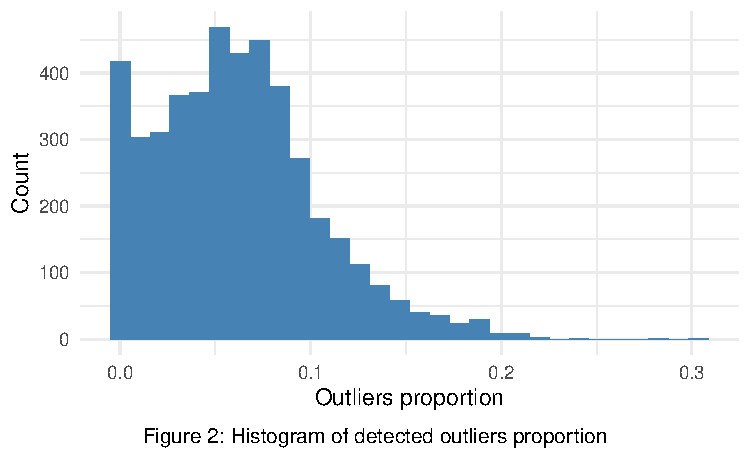
\includegraphics{new_header_format_files/figure-latex/unnamed-chunk-9-1} \end{center}

\end{CodeChunk}

Three winsorization methods are applied on users data with detected
outliers, the summary of fitted users before and after winsorization is
presented in Table 6. The results show that the proportion of fitted
users data after winsorization are increased significantly, where the
mean has the highest proportion, followed by median and then the
quantile-bases method which are consistent with the findings of the
simulation study. The Chi-square test of independence shows that there
are significant association between the status of users data (i.e fitted
by exponential distribution) before and after winsorization at 0.05
level of significance,which reveal that insignificant number of the
exponential fitted users data before winsorization has been alternated
to be not fitted by exponential after winsorization has been conducted.

\begin{CodeChunk}
\begin{table}[H]

\caption{\label{tab:unnamed-chunk-10}Summary of fitted users data before and after winsorization by exponential distribution}
\centering
\begin{tabular}[t]{l|l|l|l|l}
\hline
\multicolumn{1}{c|}{ } & \multicolumn{1}{c|}{ } & \multicolumn{3}{c}{After Outliers Winsorization} \\
\cline{3-5}
Statistics & Before & Mean & Median & Quantile-based\\
\hline
\cellcolor{gray!6}{Proportion of fitted data} & \cellcolor{gray!6}{0.31} & \cellcolor{gray!6}{0.67} & \cellcolor{gray!6}{0.61} & \cellcolor{gray!6}{0.56}\\
\hline
Chi-square test & - & 1011.42 & 1311.84 & 1632.54\\
\hline
\cellcolor{gray!6}{p-value} & \cellcolor{gray!6}{-} & \cellcolor{gray!6}{0.00} & \cellcolor{gray!6}{0.00} & \cellcolor{gray!6}{0.00}\\
\hline
\end{tabular}
\end{table}

\end{CodeChunk}

\hypertarget{conclusions}{%
\section{Conclusions}\label{conclusions}}

Outliers are more likely to exist as the data are generated from a
variety of phenomena and activities with varying characteristics and
dimensions. As a result, detecting and dealing with it will be a
constant problem. Therefore, its detection and handling will be an
ongoing challenge.

This article addressed what seems to be a plain winsorization techniques
to handle outliers via simulation study. The findings reveal that the
nature of treated data including its distribution, sample size,
percentage of outliers are vital factors in this process output.

Because of its popularity and simplicity, we have used Tukey's method ,
however it is expected that other outlier identification methods would
find different outliers. As a result, other outliers identification
procedures should be utilized to winsorizate the common identified
outliers.

\pagebreak

\textbf{REFERENCES}

Abuzaid AH, Mohamed IB and Hussin AG (2012). Boxplot for Circular
Variables. Computational Statistics. 27 (3), 381-392.

Almeroth KC and Ammarm MH (1996). Collecting and Modeling the Join/Leave
Behavior of Multicast Group Members in the MBone. In Proceedings of
International Symposium on High Performance Distributed Computing
(HPDC).

Babu GJ, Padmanabhan AR, and Puri ML (1999). Robust One-way ANOVA under
Possibly Non Regular Conditions. Biometrical Journal, 41: 321-339.

Chetlapalli V, Iyer KSS and Agrawal H (2020) Modelling time-dependent
aggregate traffic in 5G networks. Telecommun Syst 73, 557-575.
\url{https://doi.org/10.1007/s11235-019-00629-w}

Dominguesa R, Filipponea M, Michiardia P and Zouaouib J. (2018) A
Comparative Evaluation of Outlier Detection Algorithms: Experiments and
Analyses, Pattern Recogn.74: 406-421.

Ekezie DD and Ogu AI (2013) Statistical Analysis/Methods of Detecting
Outliers in Univariate Data in A Regression Analysis Model.
International Journal of Education and Research, 1(5): 1-24.

Frey B (2018). The SAGE encyclopedia of educational research,
measurement, and evaluation (Vols. 1-4). Thousand Oaks,, CA: SAGE
Publications, Inc.~doi: 10.4135/9781506326139

Frost J (2020). Hypothesis testing: An intuitive guide for making data
drives decisions. Statistics by Jim Publishing State College,
Pennysalvia, U.S.A.

Hoaglin DC, Iglewicz B, Tukey JW (1986) Performance of some resistant
rules for outlier labeling. J Am Stat Assoc 81(396):991-999

Hubert M, Rousseeuw PJ, and Van Aelst S (2008). High-breakdown Robust
Multivariate Methods. Statistical Science, 23(1): 92-119.

Lix LM and Keselman HJ (1998). To Trim or Not to Trim: Tests of Location
Equality under Heteroscedasticity and Non-normality. Educational and
Psychological Measurement, 115: 335-363.

Preparata F, Shamos M (1988) Computational Geometry: an Introduction,
Springer-Verlag, Berlin.

Saeger T, Kleven B, Otero I, Wallace M and Ziglar R(2016) Outlier
Labeling Method for Univariate Data for Module Test and Die Sort. IEEE
transactions on semiconductor manufacturing, 29 (4): 330-335.

Shimizu Y (2022) Multiple Desirable Methods in Outlier Detection of
Univariate Data With R Source Codes. Front. Psychol. 12:819854.

Sripanidkulchai K, Maggs B, and Zhang H. (2004). An analysis of live
streaming workloads on the internet. In Proceedings of the 4th ACM
SIGCOMM conference on Internet measurement (IMC '04). Association for
Computing Machinery, New York, NY, USA, 41-54.
\url{DOI:https://doi.org/10.1145/1028788.1028795}

Tukey JW (1977) Exploratory data analysis. Addison-Wesley, Reading.

Tukey JW (1959). A survey of sampling from contaminated distributions.
Princeton, New Jersey: Princeton University.

Wilcox RR (2003). Applying Contemporary Statistical Techniques. Academic
Press: San Diego, CA.

Yusof ZM, Othman AR, and Syed Yahaya SS (2013). Robustness of Trimmed F
Statistics when Handling Nonnormal Data. Malaysian Journal of Science,
32(1): 73-77.




\end{document}
